%
%
\comment{
\begin{itemize}
	\item in cmps where all data are cache lines and there is a limited number of outstanding requests, and incoming data each has a tag to indicate which it is. processors can resolve exactly what to do with this data.
	\item we want to have streams of data so we can either tag each packet with a order id and add reordering buffers which may be huge and impossible to size, or we can constrain the NoC such that packets always arrive in-order.
	\item this means that we must use deterministic routing algorithms -- we use dor, and we can use VCs but each message class is limited to using only a single VC.
	\item give formal notation for the constraint on VCs -- data originating at a src and going to a dest must stay on the same VC.
	\item an average user should not be aware that the NoC exists: it is simply a portal in which s/he can throw data in and expect it to arrive at the other end.
	\item usually people don't care how efficiently they are actually using their interconnect resources.
	\item advanced designers will want to make best use of the NoC bandwidth/power and can therefore optimize the data size before inserting into the NoC and write custom interfaces in which case they would want to know the min flit width and min packet width -- the former is relevant for latency-insensitive and the latter is relevant for latency-sensitive.
	\item we can use the NoC both in latency-sensitive mode when we establish a permanent channel between two modules (and here we have the advantage of parallel compilation, freedom of placement etc)
	\item or latency-insensitive mode for everything else when we cannot map communication into non-intersecting paths on the NoC.
\end{itemize}
}
%
%

Fig.~\ref{classification} shows the two possibilities of synchronous design styles, as well as two communication protocols that are common in FPGA designs.
%The two design styles are ``latency-insensitive", and ``latency-sensitive". 
In a latency-insensitive system, the design consists of \textit{patient} modules that can be stalled, thus allowing the interconnect between those modules to have arbitrary delay~\cite{Carloni2002}.
Latency-sensitive design, on the other hand, does not tolerate variable latency on its connections, and assumes that its interconnect always has a fixed latency.
In this section we investigate how to map applications that belong to either design style (and any communication protocol) onto the NoC; Fig.~\ref{sys} illustrates this.
We are effectively augmenting the FPGA with a wide stallable network of buffered interconnect that can do flexible switching -- how can we best leverage that new interconnection resource for different design styles? 
And can this embedded NoC be used for both latency insensitive/sensitive design styles, and both communication protocols?

%
\figvs{1}{zl_latency}{trim = 1.7cm 2.4cm 1.7cm 2.0cm, clip}{Zero-load latency of the embedded NoC (including FabricPorts) at different fabric frequencies. Latency is reported as the number of cycles at each frequency. The number of hops varies from 1 hop (minimum) to 7 hops (maximum -- chip diagonal).}
%

%
\figvs{1}{classification}{}{Design styles and communication protocols.}
%

%
\figvs{1}{sys}{}{Mapping latency-sensitive and latency-insensitive systems onto an embedded NoC. We reserve \textit{Permapaths} on the NoC to guarantee a fixed latency and perfect throughput for a latency-sensitive application. For latency-insensitive systems, modules must be encapsulated with wrappers to add stall functionality.}
%


%
%--------------------------------------------------------------------------------------------------------
\subsection{Packet Ordering and Dependencies}
%--------------------------------------------------------------------------------------------------------
%

%
%--------------------------------------------------------------
\subsubsection{Ordering}
%--------------------------------------------------------------
%

Packet-switched NoCs like the one we are using were originally built for chip multiprocessors (CMPs).
CMPs only perform \textbf{memory-mapped} communication; most transfers are cache lines or coherency messages.
Furthermore, processors have built-in mechanisms for reordering received data, and NoCs are typically allowed to reorder packets.
%do not guarantee that packets will arrive in order.

With FPGAs, memory-mapped communication can be one of two main things: (1) Control data from a soft processor that is low-bandwidth and latency-critical -- a poor target for embedded NoCs, or (2) Communication between design modules and on-chip or off-chip memory, or PCIe links -- high bandwidth data suitable for our proposed NoC.
Additionally, FPGAs are very good at implementing \textbf{streaming}, or data-flow applications such as packet switching, video processing, compression and encryption.
These streams of data are also prime targets for using our high-bandwidth embedded NoC.
Crucially, neither memory-mapped nor streaming applications tolerate packet reordering on FPGAs, nor do FPGAs natively support it.
While it may be possible to design reordering logic for simple memory-mapped applications, it becomes \textit{impossible} to build such logic for streaming applications without hurting performance -- we therefore choose to restrict the embedded NoC to perform in-order data transfers only.
Specifically, an NoC is not allowed to reorder packets on a single connection.
%
\begin{defn}
A \textbf{connection} (\textbf{s}, \textbf{d}) exists between a single source (\textbf{s}) and its downstream destination (\textbf{d}) to which it sends data.
\end{defn}
%
\begin{defn}
A \textbf{path} is the sequence of links from \textbf{s} to \textbf{d} that a flit takes in traversing an NoC.
\end{defn}
%

There are two causes of packet reordering.
Firstly, an adaptive route-selection algorithm would always attempt to choose a path of least contention through the NoC; therefore two packets of the same source and destination (same connection) may take different paths and arrive out of order.
Secondly, when sending packets (on the same connection) but different VCs, two packets may get reordered even if they are both taking the same path through the NoC.

To solve the first problem, we only use routing algorithms, in which routes are the same for all packets that belong to a connection.
%
\begin{cond}
\label{routing_constraint}
The same \textbf{path} must be taken by all packets that belong to the same \textbf{connection}.
\end{cond}
%
%
Deterministic routing algorithms such as dimension-ordered routing~\cite{dally_book} fulfill Condition~\ref{routing_constraint} as they always select the same route for packets on the same connection.
%


Eliminating VCs altogether would fix the second ordering problem; however, this is not necessary.
VCs can be used to break message deadlock, merge data streams (Fig.~\ref{merge}), alleviate NoC congestion and may be also used to assign packet priorities thus adding extra configurability to our NoC -- these properties are desirable.
We therefore impose more specific constraints on VCs such that they may still be used on FPGA NoCs.
%
\begin{cond}
All packets belonging to the same \textbf{connection} must use the same VC.
\end{cond}
%


To do this in NoC routers is simple.
Normally, a packet may change VCs at every router hop -- VC selection is done in a VC allocator~\cite{dally_book}.
We replace this VC allocator with a lightweight VC \textit{facilitator} that cannot switch a packet between VCs; instead, it inspects a packet's input VC and stalls that packet until the downstream VC buffer is available.
At the same time, other connections may use other VCs in that router thus taking advantage of multiple VCs.


%
%--------------------------------------------------------------
\subsubsection{Dependencies and Deadlock}
%--------------------------------------------------------------
%

\begin{figure}[t]
\centering
\subfloat[Standard FabricPort output.]{
   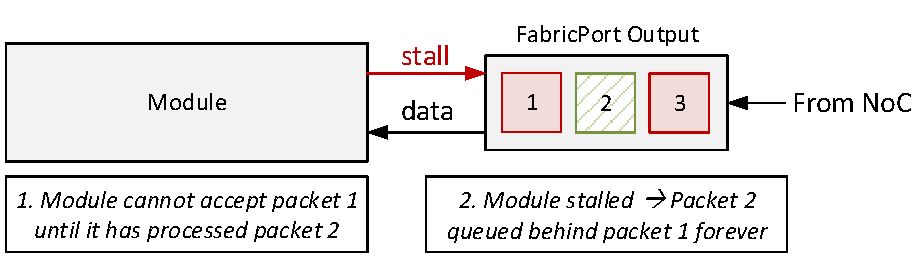
\includegraphics[width=0.9\columnwidth,keepaspectratio]{images/deadlock}
   \label{deadlock}
 }
 \\
\subfloat[Deadlock-free FabricPort output.]{
   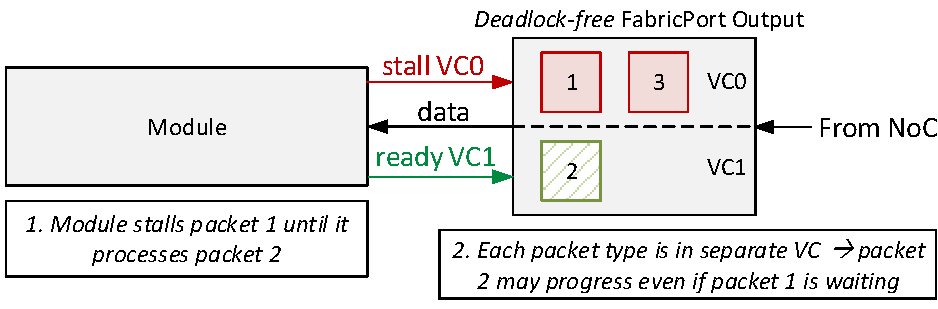
\includegraphics[width=0.9\columnwidth,keepaspectratio]{images/nodeadlock}
   \label{nodeadlock}
 }
\caption{Deadlock can occur if a dependency exists between two message types going to the same port. By using separate VCs for each message type, this deadlock can be broken thus allowing two dependent message types to share a FabricPort output.}
\label{dead}
\end{figure}


Two \textit{message types} may not share a standard FabricPort output (Fig.~\ref{fpout}) if a dependency exists between the two message types.
An example of dependent message types can be seen in video processing IP cores: both control messages (that configure the IP to the correct resolution for example) and data messages (pixels of a video stream) are received on the same port~\cite{altera_vip}.
An IP core may not be able to process the data messages correctly until it receives a control message.

Consider the deadlock scenario in Fig.~\ref{deadlock}.
The module is expecting to receive packet 2 but gets packet 1 instead; therefore it stalls the FabricPort output and packet 2 remains queued behind packet 1 forever.
To avoid this deadlock, we can send each message type in a different VC~\cite{Sorin2011}.
Additionally, we created a deadlock-free FabricPort output that maintains separate paths for each VC -- this means we duplicate the aFIFO and DEMUX units for each VC we have.
There are now two separate ``ready" signals; one for each VC, but there is still only one data bus feeding the module. 
The module can therefore \textit{either} read from VC0 or VC1.
Fig.~\ref{nodeadlock} shows that even if there is a dependency between different messages, they can share a FabricPort output provided each uses a different VC.
%
\begin{cond}
When multiple message types can be sent to a FabricPort, and a dependency exists between the message types, each type must use a different VC.
\end{cond}
%

%
%---------------------------------------------------------------------------------------------------------
\subsection{Latency-Insensitive Design with NoC}
%---------------------------------------------------------------------------------------------------------
%

Latency-insensitive design is a design methodology that decouples design modules from their interconnect by forcing each module to be \textit{patient}; that is, to tolerate variable latency on its inputs~\cite{Carloni2002}.
This is typically done by encapsulating design modules with wrappers that can stall a module until its input data arrives.
This means that a design remains functionally correct, by construction, regardless of the latency of data arriving at each module.
The consequence of this latency tolerance is that a CAD tool can automatically add pipeline stages (called \textit{relay stations}) invisibly to the circuit designer, late in the design compilation and thus improve frequency without extra effort from the designer~\cite{Carloni2002}.

Our embedded NoC is effectively a form of latency-insensitive interconnect; it is heavily pipelined and buffered and supports stalling.
We can therefore leverage such an NoC to interconnect patient modules of a latency-insensitive system as illustrated in Fig.~\ref{sys}. 
Furthermore, we no longer need to add relay stations on connections that are mapped to NoC links, avoiding their overhead.

%
\figvs{0.96}{li_wrappers_overhead}{trim = 1.5cm 3.7cm 1.5cm 3.45cm, clip}{Area and frequency of latency-insensitive wrappers from~\cite{Murray2014} (original), and optimized wrappers that take advantage of NoC buffering (NoC-compatible).}
%

Previous work that investigated the overhead of latency-insensitive design on FPGAs used FIFOs at the inputs of modules in the stall-wrappers to avoid throughput degradation whenever a stall occurs~\cite{Murray2014}.
When the interconnect is an embedded NoC; however, we already have sufficient buffering in the NoC itself (and the FabricPorts) to avoid this throughput degradation, thus allowing us to replace this FIFO -- which is a major portion of the wrapper area -- by a single stage of registers.
We compare the area and frequency of the original latency-insensitive wrappers evaluated in~\cite{Murray2014}, and the NoC-compatible wrappers in Fig.~\ref{li_wrappers_overhead} for wrappers that support one input and one output and a width between 100 bits and 600 bits.
As Fig.~\ref{li_wrappers_overhead} shows, the lightweight NoC-compatible wrappers are 87\% smaller and 47\% faster.

We envision a future latency-insensitive design flow targeting embedded NoCs on FPGAs.
Given a set of modules that make up an application, they would first be encapsulated with wrappers, then mapped onto an NoC such that performance of the system is maximized.


%
%---------------------------------------------------------------------------------------------------------
\subsection{Latency-Sensitive Design with NoC\\(Permapaths)}
%---------------------------------------------------------------------------------------------------------
%

%need to introduce latency insensitive design
Latency-sensitive design requires predictable latency on the connections between modules.
That means that the interconnect is not allowed to insert/remove any cycles between successive data.
Prior NoC literature has largely focused on using circuit-switching to achieve quality-of-service guarantees but could only provide a bound on latency rather than a guarantee of fixed latency~\cite{Goossens2005}.
We analyze the latency and throughput guarantees that can be attained from an NoC, and use those guarantees to determine the conditions under which a latency-sensitive system can be mapped onto a packet-switched embedded NoC.
Effectively, our methodology creates permanent paths with predictable latencies (Permapaths) on our packet-switched embedded NoC.

%
%----------------------------------------------------------------------------
\subsubsection{Latency and Throughput Guarantees}
\label{subsec_guarantees}
%----------------------------------------------------------------------------
%


To ensure that the NoC doesn't stall due to unavailable buffering, we size NoC buffers for maximum throughput, so that we never stall while waiting for backpressure signals within the NoC.
This is well-studied in the literature and is done by sizing our router buffers to cover the \textit{credit round-trip latency}~\cite{dally_book} -- for our system, a buffer depth of 10 suffices.



Fig.~\ref{zl_xput} plots the throughput between any source and destination on our NoC in the absence of contention.
The NoC is running at 1.2~GHz with 1-flit width; therefore, if we send 1 flit each cycle at a frequency lower than 1.2~GHz, our throughput is always perfect -- we'll receive data at the same input rate (one flit per cycle) on the other end of the NoC path. 
In fact, the NoC connection acts as a simple pipelined wire; the number of pipeline stages are equivalent to the zero-load latency of an NoC path; however, it is irrelevant because that latency is only incurred once at the very beginning of data transmission after which data arrives on each fabric clock cycle.
We call this a \textbf{Permapath} through the NoC: a path that is free of contention and has perfect throughput.
As Fig.~\ref{zl_xput} shows, we can create Permapaths of larger widths provided that the input bandwidth of our connection does not exceed the NoC port bandwidth of 22.5~GB/s.
This is why throughput is still perfect with 4~flits$\times$300~MHz for instance.
To create those Permapaths we must therefore ensure two things:
%
\begin{cond}
(Permapaths)
The sending module data bandwidth must be less than or equal to the maximum FabricPort input bandwidth.
\end{cond}
%
\begin{cond}
\label{traf_cond}
(Permapaths)
No other data traffic may overlap the NoC links reserved for a Permapath to avoid congestion delays on those links.
\end{cond}
%
Condition~\ref{traf_cond} be determined statically since our routing algorithm is deterministic; therefore, the mapping of modules onto NoC routers is sufficient to identify which NoC links will be used by each module.


%
\figvs{0.96}{zl_xput}{trim = 1.5cm 3.7cm 1.5cm 3.45cm, clip}{Zero-load throughput of embedded NoC path between any two nodes, normalized to sent data. A throughput of ``1" is the maximum; it means that we receive $i$ flits per cycle, where $i$ is the number of flits we insert in the FabricPort each cycle.}
%

%
%---------------------------------------------------------------------------------------------------------
\subsection{Multicast, Reconvergence and Feedback}
%---------------------------------------------------------------------------------------------------------
%

%
\figvs{0.8}{multicast}{}{Aspects of complex FPGA applications.}
%

A complex FPGA application may include multicast, reconvergence and feedback as shown in Fig.~\ref{multicast} -- we discuss these aspects briefly here but leave the in-depth analysis for future work.
Prior NoC research has shown that packet-switched routers can be augmented with multicast capability at very low area overhead~\cite{Enright2008}.
As for reconvergence, the two branches of a reconvergent path may have different latencies on the embedded NoC with different implications for latency-sensitive and latency-insensitive systems.
A latency-sensitive system may become functionally incorrect in that case; the designer must therefore ensure that the paths are balanced.
For a latency-insensitive system functional correctness is guaranteed but throughput degradation may occur if latencies of the two paths differ by a large amount; prior work has investigated path balancing for latency-insensitive systems~\cite{Lu2003}.
Balancing can be done by selecting two paths of the same length through the NoC (hence same latency) and using registers in the FPGA fabric for fine-grained latency adjustment.
Feedback paths are also tricky to implement on embedded NoCs; this stems from the fact that these connections are typically latency-critical and require very low latency so as not to impede throughput.

While some of these connections can be mapped onto the NoC, not all of them have to be; the embedded NoC is not meant to be an interconnect capable of connecting everything on the FPGA; rather a flexible low-cost (but high bandwidth) interconnect resource that \textit{augments} the current FPGA traditional interconnect. 
Remember that the embedded NoC is 1.3\% of FPGA core area while the FPGA's traditional interconnect accounts for \til50\%~\cite{Lewis2013}.
Traditional interconnect can still be used for latency-critical connections while the embedded NoC can be leveraged for connections on which timing closure is difficult or those that require buffering, stallability, or heavy switching.



%
%
